% Evitar que los bloques de figuras estiren los espacios entre párrafos.
\raggedbottom

\chapter{Introducción}
\label{sec:introduction}

% Estructura (revisión docente): macro (rubro, 2 párr.) → micro (San Miguel,
% 2 párr.) → etapa estudiada → concepto de solución → ¿qué? ¿quién? ¿con qué?
% ¿para qué? Sin mediciones propias (van en 1.3 y 4.0).

% --- MACRO 1: el pan y las panaderías ---------------------------------------
% [CONSERVA]
\textcite{ribet2025bread} y \textcite{allipour2023bread} describen el pan
como un alimento básico y como uno de los productos de cereales de mayor
consumo en el mundo. \textcite{ribet2025bread} señalan, además, que el pan
aporta no menos del 10\,\% de los requerimientos energéticos de la población
mundial. En ocho países de América Latina, sin incluir a Bolivia,
\textcite{kovalskys2022breakfast} registraron que el grupo de panes blancos,
bollos y tortillas fue el de mayor consumo en el desayuno de la población
urbana (60\,\%). La elaboración de pan abarca desde plantas industriales
hasta talleres artesanales de pequeña escala, como muestran
\textcite{drozd2023systemic} en Polonia y \textcite{esponda2023saberes} en
México. En los talleres documentados en Chiapas y Barcelona, la medición de
los ingredientes queda a cargo de quien elabora el pan.
\textcite{esponda2023saberes} recogieron el testimonio de una panadera que
emplea el puño de la mano como patrón de medida, y \textcite{rogerio2018sabor}
observó el pesaje en básculas digitales previo al amasado, con errores
ocasionales que la panadera corrige durante el proceso.
% VERIFICAR en PDF. Páginas de respaldo (no se imprimen): cifra del 10 % en
% Ribet et al. (por confirmar). Allipour-Birgani et al. p. 20. Kovalskys et al.
% p. 1099. Esponda-Pérez et al. pp. 13--15 y 38. Rogério pp. 58 y 169.

% --- MACRO 2: Bolivia y Santa Cruz -------------------------------------------
% [AJUSTE] Se unen los dos párrafos en uno y se retira la figura de
% producción de trigo por departamento (las cifras se conservan en el texto).
% Motivo: el docente pide 1–2 párrafos macro, y para una panadería el dato
% más directo es el de unidades productivas. La figura retirada pasa a 4.0 o
% a anexo [DECISIÓN].
De acuerdo con \textcite{fao2026fbs}, el suministro de trigo y productos
derivados para alimentación humana en Bolivia se situó entre 43,76 y
60,46~kg por persona y año en el período 2018--2023. Según el
\textcite{mdpyep2023trigo}, la producción nacional de trigo alcanzó
310\,730~t en 2022, de las cuales Santa Cruz aportó 233\,769~t, el
75,2\,\% del total. El mismo informe registra importaciones de harina de
trigo por 145\,151~t en 2022, con Argentina como principal país de origen,
y señala que la Empresa de Apoyo a la Producción de Alimentos (EMAPA)
ejecuta la política de subvención a los derivados del trigo establecida por
el Decreto Supremo 255, con la cual los precios al consumidor se mantienen
relativamente estables. En el registro de comercio de 2022, la industria de
productos de panadería comprendía 354 unidades productivas formales. La
Figura~\ref{fig:empresas_panaderia_departamento} presenta la distribución de
esas unidades por departamento: Santa Cruz registró 126 unidades, el
36\,\%, seguida de La Paz con 86 (24\,\%) y de Cochabamba con 83 (23\,\%).
Santa Cruz concentra, por tanto, la mayor parte de la producción nacional de
trigo y la mayor proporción de las unidades productivas de panadería
registradas en el país.
% VERIFICAR: valor 2023 de FAOSTAT (43,76 kg). Páginas de respaldo del MDPyEP
% (no se imprimen): producción y Santa Cruz pp. 25--26 y 31 (Tabla 2).
% Importación pp. 81--82. EMAPA y DS 255 pp. 20 y 86. Unidades productivas
% pp. 58--59 (Tabla 9).
% [VERIFICAR] «relativamente estables»: redacción.md marca el adverbio como
% vago; se conserva porque reproduce la valoración del informe (p. 86).
% Confirmar la expresión en la fuente.
% NOTA: en la Tabla 2 de la fuente, la suma departamental (310 154 t) no
% coincide con el total (310 730 t). El MDPyEP indica 99 % de origen argentino
% y 93 mil t para 2022, cifra que no coincide con el total de 145 151 t; por
% eso se escribe «principal país de origen» sin porcentaje. Las 354 unidades
% son solo las registradas formalmente y no incluyen panaderías informales.
% VERIFICAR: la Tabla 9 de la fuente no indica el año.

\begin{figure}[H]
    \centering

    {\setlength{\fboxsep}{6pt}
    \fbox{%
        % Unidades productivas de elaboración de productos de panadería por
% departamento. Adaptado de MDPyEP (2023), Tabla 9 (fuente original: SIIP,
% procesado por DGAPIyEP). Valores sin modificar.
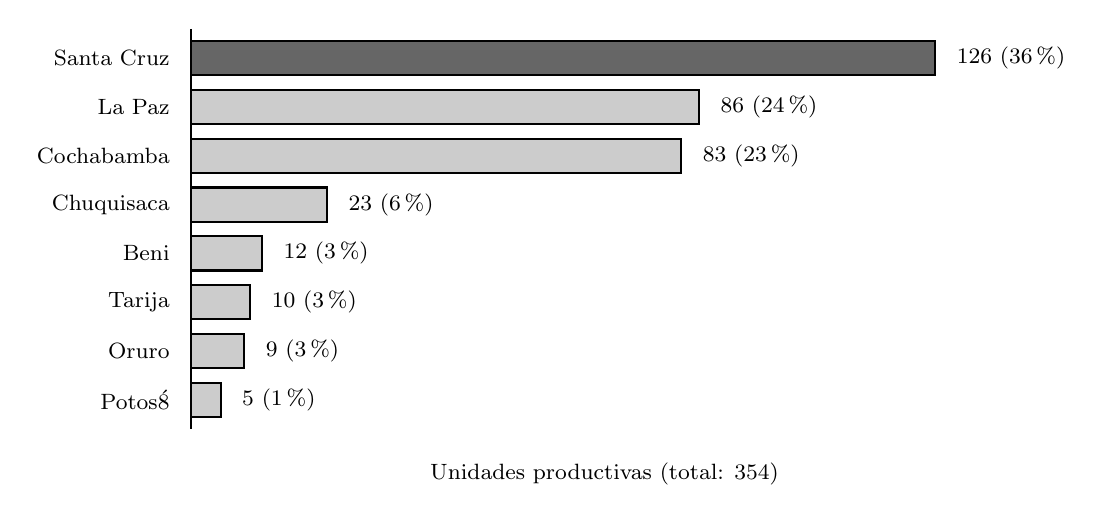
\begin{tikzpicture}[
    x=0.075cm,
    y=-0.62cm,
    barra/.style={draw, fill=black!20, thick},
    destacada/.style={draw, fill=black!60, thick},
    etiqueta/.style={font=\footnotesize, anchor=east},
    valor/.style={font=\footnotesize, anchor=west}
]

% Departamento / unidades productivas / participación
\foreach \dep/\val/\por [count=\i] in {
    Santa Cruz/126/36,
    La Paz/86/24,
    Cochabamba/83/23,
    Chuquisaca/23/6,
    Beni/12/3,
    Tarija/10/3,
    Oruro/9/3,
    Potosí/5/1}
{
    \ifnum\i=1
        \draw[destacada] (0,\i-0.35) rectangle (\val,\i+0.35);
    \else
        \draw[barra] (0,\i-0.35) rectangle (\val,\i+0.35);
    \fi
    \node[etiqueta] at (-2,\i) {\dep};
    \node[valor] at (\val+2,\i) {\val\ (\por\,\%)};
}

% Eje
\draw[thick] (0,0.4) -- (0,8.6);
\node[font=\footnotesize, anchor=north] at (70,9.1)
    {Unidades productivas (total: 354)};

\end{tikzpicture}

    }}

    \caption{Unidades productivas de panadería por departamento.}
    \label{fig:empresas_panaderia_departamento}

    \vspace{0.2em}
    {\footnotesize Fuente: Adaptado de \textcite{mdpyep2023trigo}.}

\end{figure}

% Figura retirada de la Introducción (trasladar a 4.0 o anexo):
% % Producción de trigo por departamento, año 2022. Adaptado de MDPyEP (2023),
% Tabla 2 (fuente original: INE con base en OAP--MDRyT). Valores sin modificar.
% NOTA: en la fuente, la suma de los departamentos (310 154 t) no coincide con
% el total publicado (310 730 t), y Potosí figura con 18 655 t y 6,2 %
% (18 655 t equivalen a 6,0 %). Se reproducen los valores tal como constan.
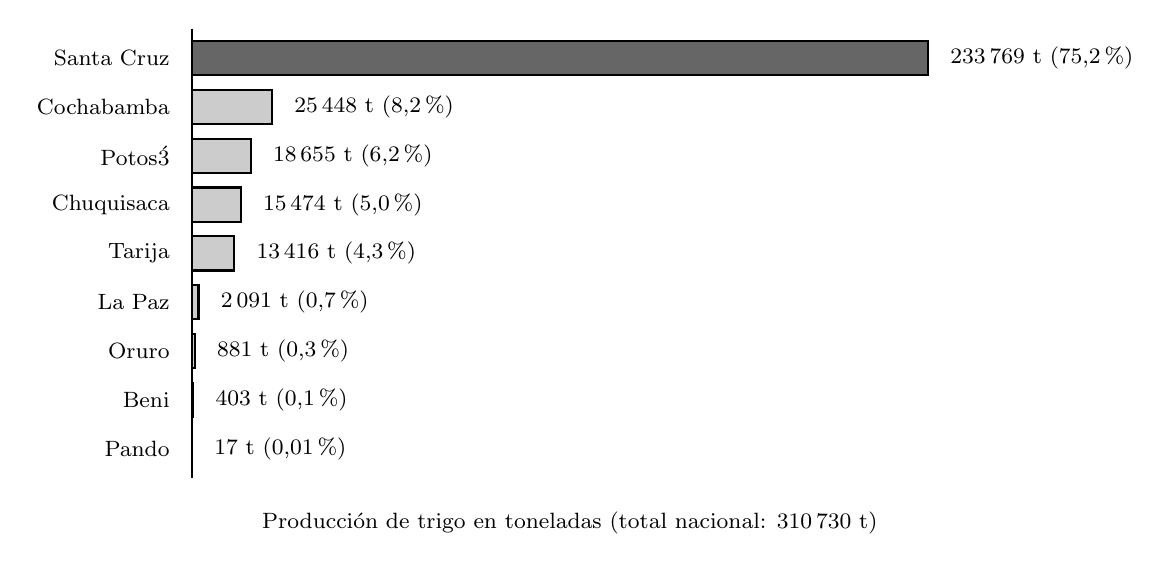
\begin{tikzpicture}[
    x=0.04cm,
    y=-0.62cm,
    barra/.style={draw, fill=black!20, thick},
    destacada/.style={draw, fill=black!60, thick},
    etiqueta/.style={font=\footnotesize, anchor=east},
    valor/.style={font=\footnotesize, anchor=west}
]

% Departamento / producción (miles de t, solo para la longitud de barra) / etiqueta de producción / participación
\foreach \dep/\val/\txt/\por [count=\i] in {
    Santa Cruz/233.769/233\,769/75{,}2,
    Cochabamba/25.448/25\,448/8{,}2,
    Potosí/18.655/18\,655/6{,}2,
    Chuquisaca/15.474/15\,474/5{,}0,
    Tarija/13.416/13\,416/4{,}3,
    La Paz/2.091/2\,091/0{,}7,
    Oruro/0.881/881/0{,}3,
    Beni/0.403/403/0{,}1,
    Pando/0.017/17/0{,}01}
{
    \ifnum\i=1
        \draw[destacada] (0,\i-0.35) rectangle (\val,\i+0.35);
    \else
        \draw[barra] (0,\i-0.35) rectangle (\val,\i+0.35);
    \fi
    \node[etiqueta] at (-4,\i) {\dep};
    \node[valor] at (\val+4,\i) {\txt~t (\por\,\%)};
}

% Eje
\draw[thick] (0,0.4) -- (0,9.6);
\node[font=\footnotesize, anchor=north] at (120,10.1)
    {Producción de trigo en toneladas (total nacional: 310\,730~t)};

\end{tikzpicture}

% \label{fig:produccion_trigo_departamento}
% Fuente: Adaptado de \textcite{mdpyep2023trigo}.

% --- MICRO 1: la panadería ---------------------------------------------------
% [AJUSTE] + [CONFIRMAR] La segunda oración necesita los datos de la
% entrevista. Redacción realista para un establecimiento artesanal de barrio;
% no imprimir los corchetes sin confirmar.
La Panadería San Miguel, ubicada en Santa Cruz de la Sierra, constituye el
caso de estudio del proyecto.
% [CONFIRMAR] Oración pendiente de la entrevista; no se imprime hasta tener
% los datos: «Se trata de un establecimiento de elaboración artesanal que
% funciona desde [AÑO] y que vende la producción en el propio local y a
% [CLIENTES: vecinos de la zona, tiendas de barrio u otros].»
La panadería elabora pan casero, marraqueta y pan francés, además de una masa
común destinada a empanadas y rollos de queso. Los sábados, la producción
incluye también cuñapé, masaco y pan de arroz.
% Respaldo (no se imprime): paredes2026registros (productos registrados) y
% paredes2026sabado (productos del sábado, pendiente de contraste).
% A-001 abierto: «artesanal» figura en el título actual; mantener la
% coherencia si el título cambia.

% --- MICRO 2: mecanización parcial ----------------------------------------
% [NUEVO] Dato estable de PROJECT_CONTEXT §1. Una sola oración, sin flujos ni
% mediciones (criterio docente); el detalle de equipos va en 4.0.
La panadería cuenta con mecanización parcial: el amasado, la división de la
masa y la cocción se realizan con equipos, mientras que la dosificación de
harina se realiza de forma manual con una balanza digital.

% --- Proceso general y etapa estudiada ----------------------------------------
% [AJUSTE] Se retira la cláusula final («etapa que en la Panadería San Miguel
% se realiza de forma manual»), ya dicha en el párrafo anterior.
\textcite{cauvain2015technology} describe que la elaboración de pan
comprende la preparación y dosificación de ingredientes, el mezclado y
amasado, la división y formado de la masa, la fermentación y la cocción, con
variaciones según el producto y el método empleado. La
Figura~\ref{fig:proceso_general_pan} presenta estas etapas. Dentro de ellas,
la dosificación establece la cantidad de cada ingrediente que ingresa al
proceso, y el recuadro de líneas discontinuas de la figura la delimita y
destaca la harina como la materia prima comprendida en el proyecto. El
estudio se concentra en la dosificación de harina previa al mezclado y
amasado.

\begin{figure}[H]
    \centering

    \resizebox{0.95\textwidth}{!}{%
        {\setlength{\fboxsep}{10pt}
        \fbox{%
            \begin{tikzpicture}[
    node distance=8mm and 8mm,
    >=Latex,
    block/.style={
        rectangle,
        draw,
        minimum height=1.2cm,
        text width=3.2cm,
        align=center,
        font=\small
    },
    alcance/.style={
        block,
        dashed,
        very thick,
        font=\small\bfseries
    },
    arrow/.style={
        -{Latex[width=8pt,length=6pt]},
        thick
    }
]

% -----------------------------------------------------------------
% Primera fila
% -----------------------------------------------------------------

\node (preparacion) [block]
{Preparación de\\ingredientes};

\node (dosificacion) [alcance, right=of preparacion]
{Dosificación de\\ingredientes\\
\textit{\footnotesize Alcance: harina}};

\node (mezclado) [block, right=of dosificacion]
{Mezclado y\\amasado};

\node (formado) [block, right=of mezclado]
{División y\\formado};


% -----------------------------------------------------------------
% Segunda fila
% -----------------------------------------------------------------

\node (fermentacion) [block, below=12mm of formado]
{Fermentación};

\node (horneado) [block, left=of fermentacion]
{Horneado};

\node (producto) [block, left=of horneado]
{Producto\\terminado};


% -----------------------------------------------------------------
% Conexiones
% -----------------------------------------------------------------

\draw [arrow] (preparacion) -- (dosificacion);
\draw [arrow] (dosificacion) -- (mezclado);
\draw [arrow] (mezclado) -- (formado);

\draw [arrow]
    (formado.south)
    -- ++(0,-5mm)
    -| (fermentacion.north);

\draw [arrow] (fermentacion) -- (horneado);
\draw [arrow] (horneado) -- (producto);

\end{tikzpicture}
        }}
    }

    \caption{Proceso general de elaboración del pan.}
    \label{fig:proceso_general_pan}

    \vspace{0.2em}
    {\footnotesize Fuente: Adaptado de \textcite{lim2019spc}.}

\end{figure}
% VERIFICAR: el texto cita a Cauvain y la figura a Lim y Antony. Confirmar la
% fuente real del diagrama.

% --- Concepto de solución -----------------------------------------------------
% [CONSERVA]
El proyecto adopta como concepto de solución la dosificación gravimétrica
automatizada, que utiliza el pesaje para determinar la cantidad suministrada
respecto de una cantidad objetivo. La \textcite{oiml2017r61} describe este
principio en la recomendación OIML R 61-1, referida a instrumentos
automáticos de llenado gravimétrico que integran funciones de alimentación,
pesaje, control y descarga.

% --- ¿Qué? ¿Quién? ¿Con qué? ¿Para qué? ---------------------------------------
% [AJUSTE] Reemplaza el último párrafo actual para no repetir el objetivo
% general palabra por palabra. Responde a la plantilla: qué (prototipo),
% quién (Panadería San Miguel), con qué (pesaje gravimétrico y control de la
% alimentación), para qué (cantidad de harina y duración de la dosificación).
% «con el fin de» expresa propósito, no un resultado (D-008).
En este contexto, el proyecto desarrolla un prototipo de dosificación
gravimétrica de harina para la Panadería San Miguel. El prototipo mide la
cantidad dosificada y controla la alimentación hasta la cantidad objetivo
configurada por el operario, con el fin de regular la cantidad de harina
respecto de la receta y disminuir la intervención manual y la duración de la
dosificación. El desempeño del prototipo se evalúa frente al procedimiento
manual bajo condiciones comparables.

%%%%%%%%%%%%%%%%%%%%%%%%%%%%%%%%%%%%%%%%%%%%%%%%%%%%%%%%%%%%%%%%%%%%%%%%%%%%%%%
% 1.1 METAS DE LA EMPRESA
%%%%%%%%%%%%%%%%%%%%%%%%%%%%%%%%%%%%%%%%%%%%%%%%%%%%%%%%%%%%%%%%%%%%%%%%%%%%%%%

\section{Metas de la empresa}
\label{sec:metas_empresa}

% Meta confirmada por el propietario (según el estudiante, 07/10/2026).
% PENDIENTE: registrar la comunicación personal (fecha, persona) para citarla.
% Estructura (plantilla / ref. 04): meta → por qué la etapa manual es la
% pertinente → alineación con dato de la etapa → cómo se evalúa (D-008).
La Panadería San Miguel tiene como meta completar la producción diaria de
pan en menor tiempo con el personal disponible, y conservar en cada
producto la cantidad de ingredientes establecida en la receta. Como
establecimiento con mecanización parcial, la panadería orienta esta meta a
las etapas que se realizan de forma manual.

El proyecto se alinea con esta meta en la dosificación de harina, etapa
manual previa al mezclado y amasado. En los siete ciclos registrados, este
procedimiento acumuló $411{,}9\ \mathrm{s}$, y las cargas principales con
los retornos representaron el $63{,}0$\,\% de ese tiempo
(Sección~\ref{sec:contextualizacion}). El prototipo asume la alimentación y
el ajuste final de la harina, y la duración del ciclo resultante se compara
con la del procedimiento manual bajo condiciones comparables.
% [DERIVADO] Cifras de 4.0. La comparación exige el mismo intervalo de
% medición en ambos casos (redacción.md §4: tiempo total ≠ intervención).
% [CONFIRMAR] Si la panadería informa la duración de la jornada de
% producción, agregar el porcentaje que ocupa la dosificación (indicador
% relativo pedido por el docente).

%%%%%%%%%%%%%%%%%%%%%%%%%%%%%%%%%%%%%%%%%%%%%%%%%%%%%%%%%%%%%%%%%%%%%%%%%%%%%%%
% 1.2 OBJETIVOS DE LA EMPRESA ALINEADOS AL PROYECTO
%%%%%%%%%%%%%%%%%%%%%%%%%%%%%%%%%%%%%%%%%%%%%%%%%%%%%%%%%%%%%%%%%%%%%%%%%%%%%%%

\section{Objetivos de la empresa alineados al proyecto}
\label{sec:objetivos_empresa}

% [CONFIRMAR] Cualidades realistas para un taller artesanal:
%   1–4 = variables de evaluación (PROJECT_CONTEXT §2, D-008);
%   5   = costo acorde a la escala (A-001: criterio, no afirmación de
%         bajo costo); se apoya en la tabla RUICHUAN / Trust-Long;
%   6   = limpieza y mantenimiento en el local (inocuidad y mantenibilidad
%         mencionadas por el docente; prepara RNF y estado del arte).
Para atender esta meta, la panadería requiere que la dosificación de harina
cumpla con las siguientes cualidades:

\begin{itemize}
    \item \textbf{Duración del ciclo:} el tiempo de cada ciclo de
    dosificación disminuye respecto del procedimiento manual registrado.
    \item \textbf{Menor intervención:} el operario configura la cantidad
    objetivo y repone la harina, sin cargas ni ajustes manuales en cada
    ciclo.
    \item \textbf{Correspondencia con la receta:} la cantidad dosificada
    coincide con la cantidad objetivo de cada preparación dentro de una
    tolerancia definida.
    \item \textbf{Repetibilidad:} las preparaciones de un mismo producto
    reciben la misma cantidad de harina entre ciclos y jornadas.
    \item \textbf{Costo acorde a la escala del establecimiento:} el costo del
    equipo resulta inferior al precio puesto en Bolivia de equipos
    comerciales de funcionalidad comparable.
    \item \textbf{Limpieza y mantenimiento en el local:} las partes en
    contacto con la harina se desmontan para la limpieza, y los repuestos
    están disponibles en Santa Cruz de la Sierra.
\end{itemize}

Estas cualidades orientan la determinación de requerimientos de la
Sección~\ref{sec:requerimientos}. Las cuatro primeras constituyen las
variables de la validación frente al procedimiento manual descrita en la
Sección~\ref{sec:metodologia}, y las dos últimas, los criterios de
comparación con los equipos comerciales del estado del arte.
% [DECISIÓN A-001] Si se retira «bajo costo», conservar la cualidad 5 como
% criterio de comparación, sin calificativo en el título.

%%%%%%%%%%%%%%%%%%%%%%%%%%%%%%%%%%%%%%%%%%%%%%%%%%%%%%%%%%%%%%%%%%%%%%%%%%%%%%%
% 1.3 PROBLEMA Y JUSTIFICACIÓN DEL PROYECTO
%%%%%%%%%%%%%%%%%%%%%%%%%%%%%%%%%%%%%%%%%%%%%%%%%%%%%%%%%%%%%%%%%%%%%%%%%%%%%%%

\section{Problema y justificación del proyecto}
\label{sec:problema}

% Orden: textual → Ishikawa → inconformidades → oración del problema →
% justificación. La plantilla coloca la justificación primero; aquí va
% después porque justifica un problema ya expuesto (mismo orden que el
% archivo actual). [VERIFICAR] con el docente.

La descripción del problema se presenta en tres representaciones: una
descripción textual de las condiciones registradas, un diagrama de causa y
efecto y una tabla de inconformidades. Los datos de respaldo se encuentran
en la Sección~\ref{sec:contextualizacion} y en los
Apéndices~\ref{ap:registros_campo} y~\ref{ap:tablas_dosificacion}.

%------------------------------------------------------------------------------
\subsection{Descripción textual}
\label{subsec:descripcion_textual}
%------------------------------------------------------------------------------

% [REUBICA] Párrafo retirado de la Introducción y párrafos de 1.3.1 actual,
% reorganizados como condiciones del proceso (criterio docente).
% [DERIVADO] porcentajes y s/kg (ver cabecera).

La Panadería San Miguel registró siete ciclos de dosificación manual de
harina, cinco en una jornada ordinaria y dos en una jornada de sábado, con
cantidades objetivo comprendidas entre 5,000 y 8,000~kg por ciclo
(Tabla~\ref{tab:resumen_dosificacion}). En esa muestra se identificaron las
siguientes condiciones del procedimiento:

\begin{itemize}

    \item La alimentación de harina se realiza mediante cargas sucesivas
    transportadas desde la zona de almacenamiento hasta la balanza. Las
    cargas principales y los retornos requeridos acumularon
    $259{,}7\ \mathrm{s}$, equivalentes al $63{,}0$\,\% del tiempo total
    registrado. El tiempo de la muestra equivale a
    $8{,}58\ \mathrm{s}$ por kilogramo de harina dosificada.

    \item La secuencia de cargas se repite para cada producto: tres cargas
    principales en los ciclos de pan casero y cuatro en los de marraqueta,
    con tiempos de $53{,}2$ a $54{,}2\ \mathrm{s}$ y de $64{,}9$ a
    $65{,}9\ \mathrm{s}$, respectivamente.

    \item La cantidad final se alcanza mediante un ajuste manual posterior a
    la última carga principal. En los siete ciclos, la lectura previa al
    ajuste permaneció por debajo de la cantidad objetivo, y la lectura final
    quedó entre $+0{,}011$ y $+0{,}038\ \mathrm{kg}$ por encima de ella,
    equivalente a una diferencia relativa de $0{,}14$ a $0{,}58$\,\%.

    \item El resultado del ajuste final varía entre preparaciones del mismo
    producto: en los tres ciclos de pan casero, con cantidad objetivo de
    $6{,}500\ \mathrm{kg}$, la diferencia osciló entre $+0{,}013$ y
    $+0{,}038\ \mathrm{kg}$.

    \item La balanza indica la cantidad acumulada, y la decisión de cargar,
    ajustar y detener la alimentación depende de la comparación visual entre
    esa lectura y la cantidad objetivo.
    % [VERIFICAR] Confirmar que la balanza no tiene función de límite o
    % alarma usada en planta.

\end{itemize}

% Fórmula de la plantilla: [VI] + [efecto en VD] + [condiciones] + [contexto].
En síntesis, la alimentación por cargas manuales sucesivas con ajuste final
por comparación visual produjo diferencias positivas de $0{,}14$ a
$0{,}58$\,\% respecto de la cantidad objetivo en los siete ciclos y
concentró el $63{,}0$\,\% del tiempo registrado en cargas y retornos, para
cantidades objetivo de 5,000 a 8,000~kg por ciclo, en la dosificación de
harina previa al mezclado y amasado de la Panadería San Miguel.

% [CONSERVA, rotulado] Proyección de la formulación actual (4.0).
Si el patrón registrado se repite en un escenario de 22 jornadas ordinarias
y cuatro sábados, el procedimiento acumula una proyección de
$1\ \mathrm{h}\ 59\ \mathrm{min}$ y $1{,}976\ \mathrm{kg}$ de diferencia
positiva por mes. Estos valores son cálculos derivados, no mediciones
mensuales (Sección~\ref{sec:contextualizacion}).
% [CONFIRMAR] Porcentaje respecto de la jornada (docente): requiere la
% duración de la jornada. No calcularlo con un valor supuesto.

%------------------------------------------------------------------------------
\subsection{Diagrama de causa y efecto}
\label{subsec:arbol_problemas}  % se conserva la etiqueta actual
%------------------------------------------------------------------------------

% Ishikawa con causas del árbol de problemas + condición derivada del ajuste
% final. Se omite «mano de obra» (docente: procesos, no personas) y
% «materiales» (sin datos de la harina, pendiente en 4.0). La «tolerancia de
% aceptación no definida» no se incluye hasta confirmarla con el propietario.

La Figura~\ref{fig:ishikawa_dosificacion} agrupa las causas del árbol de
problemas en cuatro categorías del procedimiento: método, entorno,
instrumento y medición. Las causas de método reúnen las cargas sucesivas,
los retornos para cargas adicionales y el ajuste final posterior a la última
carga principal. La causa de entorno corresponde a la separación entre la
zona de almacenamiento y la balanza, que requiere traslados entre ambas
zonas durante las cargas. Las causas de instrumento y medición
corresponden a la balanza, que indica la cantidad acumulada sin intervenir
en la alimentación, y a la comparación visual de esa lectura con la
cantidad objetivo. El diagrama ubica como efecto la dosificación no regulada
respecto de la cantidad objetivo y el ajuste final no estandarizado,
términos que retoma la formulación del problema de la
Sección~\ref{subsec:formulacion_problema}.

\begin{figure}[H]
    \centering

    \resizebox{0.95\textwidth}{!}{%
        {\setlength{\fboxsep}{6pt}
        \fbox{%
            % Diagrama de causa y efecto (Ishikawa) de la dosificación manual de harina.
% Elaboración propia a partir del árbol de problemas y de la descripción
% textual (Sección 1.3). Categorías del procedimiento: método, entorno,
% instrumento y medición. Se omite «mano de obra» (criterio docente:
% procesos, no personas) y «materiales» (sin datos de la harina, ver 4.0).
\begin{tikzpicture}[
    >=Latex,
    font=\footnotesize,
    categoria/.style={draw, thick, fill=black!10, minimum width=2.4cm,
        minimum height=0.7cm, align=center, font=\footnotesize\bfseries},
    efecto/.style={draw, very thick, text width=3.0cm, minimum height=2.2cm,
        align=center, font=\footnotesize\bfseries,
        execute at begin node={\hyphenpenalty=10000}},
    causa/.style={align=right, anchor=east, inner sep=1pt},
    espina/.style={-{Latex[width=7pt,length=6pt]}, very thick},
    hueso/.style={thick},
    flecha/.style={-{Latex[width=4pt,length=4pt]}}
]

% Espina central y efecto
\node[efecto] (efecto) at (12.0,0)
    {Dosificación no regulada respecto de la cantidad objetivo y ajuste
     final no estandarizado};
\draw[espina] (0,0) -- (efecto.west);

% Huesos superiores
\coordinate (mA) at (2.2,3.6);  \coordinate (mB) at (4.2,0);
\coordinate (eA) at (6.9,3.6);  \coordinate (eB) at (8.9,0);
% Huesos inferiores
\coordinate (iA) at (2.2,-3.6); \coordinate (iB) at (4.2,0);
\coordinate (dA) at (6.9,-3.6); \coordinate (dB) at (8.9,0);

\foreach \a/\b in {mA/mB, eA/eB, iA/iB, dA/dB}
    \draw[hueso] (\a) -- (\b);

\node[categoria, above=1pt of mA] {Método};
\node[categoria, above=1pt of eA] {Entorno};
\node[categoria, below=1pt of iA] {Instrumento};
\node[categoria, below=1pt of dA] {Medición};

% Causas: \t es la fracción del hueso desde la categoría hacia la espina
\foreach \t/\txt in {
    0.18/{Cargas sucesivas\\(3 o 4 por ciclo)},
    0.50/{Retornos para\\cargas adicionales},
    0.82/{Ajuste final posterior\\a la última carga}}
{
    \coordinate (p) at ($(mA)!\t!(mB)$);
    \draw[flecha] ($(p)+(-1.1,0)$) -- (p);
    \node[causa] at ($(p)+(-1.15,0)$) {\txt};
}

\foreach \t/\txt in {
    0.58/{Separación entre\\almacenamiento\\y pesaje}}
{
    \coordinate (p) at ($(eA)!\t!(eB)$);
    \draw[flecha] ($(p)+(-1.1,0)$) -- (p);
    \node[causa] at ($(p)+(-1.15,0)$) {\txt};
}

\foreach \t/\txt in {
    0.25/{Balanza de indicación sin\\control de la alimentación},
    0.70/{Preparación y puesta\\a cero en cada ciclo}}
{
    \coordinate (p) at ($(iA)!\t!(iB)$);
    \draw[flecha] ($(p)+(-1.1,0)$) -- (p);
    \node[causa] at ($(p)+(-1.15,0)$) {\txt};
}

\foreach \t/\txt in {
    0.58/{Comparación\\visual con la\\cantidad objetivo}}
{
    \coordinate (p) at ($(dA)!\t!(dB)$);
    \draw[flecha] ($(p)+(-1.1,0)$) -- (p);
    \node[causa] at ($(p)+(-1.15,0)$) {\txt};
}

\end{tikzpicture}

        }}
    }

    \caption{Diagrama de causa y efecto de la dosificación manual de harina.}
    \label{fig:ishikawa_dosificacion}

    \vspace{0.2em}
    {\footnotesize Fuente: Elaboración propia.}

\end{figure}
% [VERIFICAR] Correspondencia entre trayectos y cargas (24 cargas, 55
% trayectos; notas de campo: por confirmar).

Los efectos identificados en el árbol de problemas son la menor
disponibilidad del operario para otras actividades durante el procedimiento
y la variación de la cantidad de harina incorporada a la preparación
respecto de la cantidad objetivo. Los registros disponibles no establecen
consecuencias sobre desperdicio de harina, costo o calidad del producto.
% [DECISIÓN] Árbol de problemas: trasladar a 4.0 o anexo; su problema
% central cambia con 1.3.4 (D-004).

%------------------------------------------------------------------------------
\subsection{Tabla de inconformidades}
\label{subsec:inconformidades}
%------------------------------------------------------------------------------

% Modelo ISO/IEC 9126-1 (pedido por el docente), usado como taxonomía de
% características. Decisión del autor (07/10/2026): se usa el modelo sin
% citar la norma en el texto ni en la bibliografía.
% [PROPUESTO] Tolerancia ±0,1 % (A-004 sigue abierto hasta tu aprobación):
%   - los 7 ciclos superan 0,1 % → «no cumple» con respaldo;
%   - exige mejorar el mejor ciclo manual (0,14 %);
%   - medible con la balanza actual (indica en gramos).
%   [VERIFICAR] contrastar con las clases de exactitud de OIML R 61 y con la
%   diferencia aceptada por el panadero.

La Tabla~\ref{tab:inconformidades} relaciona las condiciones registradas
con características y subcaracterísticas de calidad. Cada fila indica la
especificación de referencia frente a la cual se evalúa la condición. Las
especificaciones de tiempo e intervención se establecen en la
Sección~\ref{sec:requerimientos}, y hasta entonces la conformidad de esas
filas permanece por determinar.

\begin{table}[H]
    \centering
    \caption{Inconformidades del procedimiento manual de dosificación de
    harina.}
    \label{tab:inconformidades}
    \footnotesize
    \setstretch{1}
    \setlength{\tabcolsep}{4pt}
    \renewcommand{\arraystretch}{1.35}

    \begin{tabularx}{\textwidth}{
        >{\raggedright\arraybackslash}p{0.19\textwidth}
        >{\raggedright\arraybackslash}X
        >{\raggedright\arraybackslash}p{0.23\textwidth}
        >{\raggedright\arraybackslash}p{0.12\textwidth}}
        \toprule[1pt]
        \textbf{Característica: subcaracterística} &
        \textbf{Condición registrada} &
        \textbf{Especificación de referencia} &
        \textbf{Evaluación} \\
        \midrule[1pt]

        Funcionalidad: exactitud &
        Diferencia positiva en los siete ciclos, de $0{,}14$ a
        $0{,}58$\,\% de la cantidad objetivo. &
        Cantidad objetivo de cada preparación con tolerancia de
        $\pm 0{,}1$\,\% (requisito propuesto). &
        No cumple \\
        \midrule

        Funcionalidad: exactitud entre ciclos &
        Pan casero, $6{,}500\ \mathrm{kg}$: diferencias de $+0{,}013$ a
        $+0{,}038\ \mathrm{kg}$ en tres ciclos. &
        Misma tolerancia para todos los ciclos de un producto. &
        No cumple \\
        \midrule

        Eficiencia: comportamiento en el tiempo &
        $8{,}58\ \mathrm{s/kg}$ en la muestra. De $53{,}2$ a
        $66{,}6\ \mathrm{s}$ por ciclo. &
        Tiempo objetivo por definir en requerimientos. &
        Por definir \\
        \midrule

        Eficiencia: utilización de recursos &
        Cargas principales y retornos: $63{,}0$\,\% del tiempo registrado. &
        Por definir en requerimientos. &
        Por definir \\
        \midrule

        Usabilidad: operabilidad &
        Alimentación, ajuste final y comprobación manuales en cada ciclo
        (Figura~\ref{fig:dfd_dosificacion}). &
        Intervención limitada a configurar la cantidad objetivo y reponer
        harina (alcance funcional). &
        No cumple \\
        \bottomrule[1pt]
    \end{tabularx}

    \vspace{0.5em}
    {\footnotesize Fuente: Elaboración propia con base en los registros de
    campo.}
\end{table}

% No usar los valores ilustrativos del docente (1000/800 und/h, 50 L, 60 g,
% −200 und). Fila de reglamento municipal del peso del pan: solo con la
% norma localizada y si regula la harina, no solo la pieza terminada.

%------------------------------------------------------------------------------
\subsection{Formulación del problema}
\label{subsec:formulacion_problema}
%------------------------------------------------------------------------------

% [DECISIÓN] Reemplaza «El operario destina…» (docente: proceso, no persona;
% tres términos en una oración; D-004 revisión requerida).
% Correspondencia con la evidencia:
%   «imprecisión»            → diferencia positiva 0,14–0,58 % en 7/7 ciclos.
%       [VERIFICAR] Por el VIM (jcgm2012vim) un sesgo sistemático es falta de
%       exactitud/veracidad, no de precisión; consultar el término.
%   «falta de estandarización» → ajuste final: 13–38 g en pan casero.
%       La secuencia de cargas SÍ se repite por producto (3 o 4 cargas,
%       tiempos con ±1 s): no afirmar que las cargas no están estandarizadas.
%   «uso no óptimo de recursos» → 63,0 % del tiempo en cargas y retornos.

El procedimiento manual de dosificación de harina de la Panadería San
Miguel no regula la cantidad dosificada respecto de la cantidad objetivo,
no estandariza el ajuste final entre preparaciones del mismo producto y
concentra el $63{,}0$\,\% del tiempo registrado en cargas y traslados
manuales.

%------------------------------------------------------------------------------
\subsection{Justificación}
\label{sec:justificacion}
%------------------------------------------------------------------------------

% [DECISIÓN] Se retira «Tecnológica» (docente: solo con tecnología nueva);
% su contenido pasa a «Operativa». «Social» se renombra «Operativa».

\subsubsection{Justificación económica}
\label{subsec:justificacion_economica}

% [CONSERVA] Primer párrafo y tabla RUICHUAN / Trust-Long, sin cambios.
El proyecto considera el costo de construcción e integración del prototipo
frente a soluciones comerciales de funcionalidad comparable. RUICHUAN se
seleccionó por el principio gravimétrico y el control automático que declara,
mientras que Trust-Long se incluyó por la operación por lotes de harina. La
Tabla~\ref{tab:comparativa_economica} presenta las características y los
precios publicados de ambas referencias.

\begin{table}[H]
    \centering
    \caption{Referencias comerciales para la evaluación económica del proyecto.}
    \label{tab:comparativa_economica}
    \footnotesize
    \setstretch{1}
    \setlength{\tabcolsep}{4pt}
    \renewcommand{\arraystretch}{1.35}

    \begin{tabularx}{\textwidth}{
        >{\raggedright\arraybackslash}p{0.28\textwidth}
        >{\raggedright\arraybackslash}X
        >{\raggedright\arraybackslash}X}
        \toprule[1pt]

        \textbf{Criterio} &
        \textbf{RUICHUAN} &
        \textbf{Trust-Long} \\
        \midrule[1pt]

        Modelo publicado &
        Serie SZC-T &
        TLP-500 / TLP-5000 \\
        \midrule

        Tipo de operación &
        Continua / por lotes &
        Por lotes \\
        \midrule

        Material declarado &
        Harina y polvos de baja fluidez &
        Harina y otros materiales pulverulentos \\
        \midrule

        Principio de dosificación &
        Pérdida de peso con celdas de carga &
        Pesaje digital y alimentación mediante tornillo \\
        \midrule

        Rango por lote publicado &
        No especificado &
        $0{,}5$--$15\ \mathrm{kg}$\textsuperscript{a} \\
        \midrule

        Nivel de automatización &
        Control automático mediante PLC &
        Operación semiautomática \\
        \midrule

        Precio publicado para una unidad &
        USD~$2\,000$ &
        USD~$2\,600$ para TLP-500 y
        USD~$3\,800$ para TLP-5000 \\
        \bottomrule[1pt]
    \end{tabularx}

    \vspace{0.5em}

    {\footnotesize
    Fuente: Elaboración propia con base en las publicaciones comerciales de
    RUICHUAN~\parencite{UnidadDosificadoraGravimetrica} y
    Trust-Long~\parencite{MaquinaLlenadoPolvo}.}
\end{table}

% [PENDIENTE] Agregar a la tabla la fila «Precio puesto en Bolivia».
%   Método (confirmar tasas con la Aduana Nacional; referencia consultada de
%   2019: GA 10 % consumo, 5 % o 0 % bienes de capital; IVA 14,94 % sobre
%   CIF + GA; verificación 1,75 % FOB; agencia 0,5–2 % CIF; CAINCO 0,03 %):
%     P_Bolivia = (FOB + flete + seguro) × (1 + GA) × 1,1494
%                 + cargos de despacho + transporte interno
%   Flete: cotización real del proveedor; no estimar.

El precio publicado no incluye los costos de importación. Para una
comparación en condiciones equivalentes, cada referencia comercial se
expresa como precio puesto en Bolivia, que suma al precio de origen el
flete, el seguro, el gravamen arancelario, el impuesto al valor agregado de
importación y los cargos de despacho aduanero.
% [VERIFICAR] Agregar la fuente normativa de los tributos de importación.

La comparación del costo documentado del prototipo con el precio puesto en
Bolivia de estas referencias, junto con las diferencias funcionales y
técnicas, establece el criterio para evaluar la condición de bajo costo.
% A-001 abierto: si se retira «bajo costo» del título, escribir «evaluar el
% costo del prototipo frente a estas referencias».

\subsubsection{Justificación Social}
\label{subsec:justificacion_social}  % se conserva la etiqueta actual

% [REUBICA] Social + segundo párrafo de Tecnológica, sin afirmaciones nuevas.
El operario encargado de la dosificación de harina en la Panadería San
Miguel constituye el beneficiario directo del proyecto. El procedimiento
registrado requiere la intervención del operario en la preparación del
pesaje, las cargas y los traslados, así como en el ajuste y la comprobación
final. La integración del pesaje con el control de la alimentación busca
reducir la intervención necesaria para alcanzar la cantidad objetivo.

El aporte del proyecto consiste en evaluar esta integración frente al
procedimiento manual en cuanto al tiempo de dosificación, la
intervención del operario, la diferencia respecto de la cantidad objetivo y
la repetibilidad. Los beneficios esperados se limitan al caso de estudio y
requieren comprobación experimental. Los registros actuales no respaldan
mejoras en salud ocupacional, empleo o calidad de vida.

%%%%%%%%%%%%%%%%%%%%%%%%%%%%%%%%%%%%%%%%%%%%%%%%%%%%%%%%%%%%%%%%%%%%%%%%%%%%%%%
% 1.4 OBJETIVOS DEL PROYECTO
%%%%%%%%%%%%%%%%%%%%%%%%%%%%%%%%%%%%%%%%%%%%%%%%%%%%%%%%%%%%%%%%%%%%%%%%%%%%%%%

\section{Objetivos del proyecto}
\label{sec:objetivos}

\subsection{Objetivo general}
\label{subsec:objetivo_general}

% [DECISIÓN] verbo + qué + para qué + con qué; cada término del «para qué»
% responde a un término de 1.3.4:
%   no regula la cantidad          → regule la cantidad dosificada
%   no estandariza el ajuste final → ajuste final automático y repetible
%   63 % en cargas y traslados     → intervención limitada a configurar y
%                                    reponer
% «con qué»: OIML R 61-1 como referencia (no «en cumplimiento»: A-006).
% «intervención limitada…» describe una función del alcance, no una mejora
% medida (D-008).

Desarrollar un prototipo automatizado de dosificación gravimétrica de harina
para la Panadería San Miguel, que regule la cantidad dosificada respecto de
una cantidad objetivo mediante un ajuste final automático y repetible, con
la intervención del operario limitada a configurar la cantidad objetivo y
reponer la harina, con base en el principio de llenado gravimétrico de la
recomendación OIML R~61-1.

\subsection{Objetivos específicos}
\label{subsec:objetivos_especificos}

% Uno por etapa del Modelo en V (revisión docente). Taller I recomienda 3–6;
% DS pide 7 → se sigue DS (DS-001).
% OE2 ← OE1 actual · OE3 ← OE2 · OE4 ← OE3 + OE6 · OE5 ← OE4 · OE6 ← OE5.

\begin{enumerate}

    \item Contextualizar el procedimiento manual de dosificación de harina de
    la Panadería San Miguel mediante el registro de cantidades objetivo,
    cantidades finales, cargas y tiempos por ciclo.

    \item Determinar los requerimientos funcionales y no funcionales del
    prototipo a partir de la contextualización, el diagrama de caja negra y
    la casa de calidad.

    \item Diseñar los modelos detallados de los subsistemas mecánico, de
    medición gravimétrica y de control del prototipo conforme a los
    requerimientos establecidos.
    % [DECISIÓN A-007] Con modelamiento: «…mediante modelos CAD y modelos
    % matemáticos del proceso de dosificación» y retirar el límite en 1.5.

    \item Implementar un prototipo funcional de dosificación gravimétrica
    automatizada conforme al diseño detallado, con un desglose documentado
    del costo de materiales, componentes, fabricación y montaje.

    \item Verificar el cumplimiento de los requerimientos funcionales y no
    funcionales del prototipo mediante pruebas de funcionamiento y frente a
    las normas de referencia identificadas.

    \item Validar el desempeño del prototipo frente al procedimiento manual de
    dosificación de harina bajo condiciones comparables.

\end{enumerate}

%%%%%%%%%%%%%%%%%%%%%%%%%%%%%%%%%%%%%%%%%%%%%%%%%%%%%%%%%%%%%%%%%%%%%%%%%%%%%%%
% 1.5 ALCANCE DEL PROYECTO
%%%%%%%%%%%%%%%%%%%%%%%%%%%%%%%%%%%%%%%%%%%%%%%%%%%%%%%%%%%%%%%%%%%%%%%%%%%%%%%

\section{Alcance del proyecto}
\label{sec:delimitacion}

% [DECISIÓN D-009] Se retiran 5–15 kg, 5 g, ±0,5 % y 50 kg. Los valores
% nuevos son [DERIVADO] o [PROPUESTO], rotulados como tales.

El proyecto comprende el desarrollo de un prototipo de dosificación
gravimétrica de harina para la Panadería San Miguel, con los siguientes
ejes de alcance:

\begin{itemize}

    \item \textbf{Alcance técnico:} subsistemas de almacenamiento,
    alimentación, pesaje gravimétrico, control y descarga de harina. La
    selección del mecanismo de alimentación, del accionamiento, de los
    sensores, del controlador y de los actuadores se define en los
    Capítulos~\ref{cap:diseno_tecnico} a~\ref{cap:diseno_detallado}.

    \item \textbf{Alcance funcional:} el operario configura la cantidad
    objetivo de harina antes de cada ciclo, y el prototipo controla la
    alimentación y el pesaje desde el inicio de la dosificación hasta
    alcanzar esa cantidad. La reposición de harina en el depósito se realiza
    de forma manual.
    % [CONSERVA] Alcances 2 y 5 actuales; «tolva» → «depósito» (A-004).

    \item \textbf{Capacidad y dimensiones:} el rango de dosificación
    comprende las cantidades objetivo registradas, de 5,000 a 8,000~kg por
    ciclo. Como requisito propuesto, la capacidad útil de almacenamiento
    cubre al menos los 36,5~kg de harina dosificados en la jornada ordinaria
    registrada, de modo que la reposición se realice una vez por jornada.
    Las dimensiones se ajustan al espacio disponible junto a la zona de
    pesaje (Figura~\ref{fig:croquis_panaderia}).
    % [CONFIRMAR] presentación de compra de la harina (tamaño de bolsa) y
    % medida del espacio disponible. Valores finales en 4.3 (A-004).

    \item \textbf{Alcance normativo:} la recomendación OIML R~61-1 se emplea
    como referencia de diseño y de verificación. El proyecto no certifica el
    cumplimiento de esta recomendación.
    % [VERIFICAR A-006] OIML R 60 (celdas de carga) y R 76 (instrumentos de
    % pesaje no automáticos): agregar al confirmar su aplicación y su fuente.
    % ISO 12100 e inocuidad: mencionadas en clase, sin fuente aún.

    \item \textbf{Alcance de pruebas:} como plan propuesto, la verificación
    comprende diez ciclos para cada cantidad objetivo de 5,000, 6,500 y
    8,000~kg, con un total de 30 ciclos. La validación compara diez ciclos
    del prototipo con diez ciclos del procedimiento manual para la cantidad
    objetivo de 6,500~kg, correspondiente al pan casero, el producto con más
    ciclos en la muestra registrada.
    % [PROPUESTO] Diez ciclos por condición para estimar la dispersión
    % (repetibilidad). Ajustar si la panadería limita los ensayos con harina
    % de producción. Los diez ciclos manuales amplían los 3 ya registrados
    % de pan casero (A-003).

    \item \textbf{Alcance temporal:} la contextualización, la determinación
    de requerimientos y el diseño se desarrollan en Diseño Superior, hasta
    diciembre de 2026. La implementación, la verificación, la validación y
    los procedimientos de operación se desarrollan en Taller de Grado~II.
    % [CONFIRMAR] fechas del semestre de Taller de Grado II; completar
    % cronograma.tex (vacío).

    \item \textbf{Alcance de usuarios:} el prototipo se dirige al personal
    encargado de la dosificación de harina en la Panadería San Miguel, y la
    validación se realiza en este establecimiento.

    \item \textbf{Alcance de limitaciones:}
    \begin{itemize}
        % [CONSERVA] Límites actuales.
        \item El proyecto no incluye la validación del prototipo en otros
        establecimientos.
        \item El proyecto no automatiza la dosificación de ingredientes
        distintos de la harina. % A-005 abierto
        \item El proyecto no automatiza el mezclado y amasado, la división y
        formado, la fermentación ni la cocción del producto.
        \item El proyecto no incluye un análisis de rentabilidad del
        establecimiento, período de recuperación de la inversión ni costos de
        producción comercial en serie.
        \item El proyecto no incluye el modelamiento matemático del sistema
        de dosificación. % A-007 abierto
    \end{itemize}

\end{itemize}

%%%%%%%%%%%%%%%%%%%%%%%%%%%%%%%%%%%%%%%%%%%%%%%%%%%%%%%%%%%%%%%%%%%%%%%%%%%%%%%
% 1.6 METODOLOGÍA DE DESARROLLO DEL PROYECTO
%%%%%%%%%%%%%%%%%%%%%%%%%%%%%%%%%%%%%%%%%%%%%%%%%%%%%%%%%%%%%%%%%%%%%%%%%%%%%%%

\section{Metodología de desarrollo del proyecto}
\label{sec:metodologia}

% Formato de la plantilla DS: enfoque → metodología(s) → etapas en formato
% «etapa → descripción». Solo Modelo en V (criterio docente). PDCA y RUP
% figuran en el ejemplo de la plantilla, pero el proyecto no los adopta;
% agregarlos solo si se aplican de verdad (p. ej., RUP para el software).
% [VERIFICAR] Fuente del Modelo en V (p. ej., VDI 2206) para la .bib.
% [PENDIENTE] Figura images/ds/modelo_v.tex (recomendada en THESIS_STRUCTURE).

El desarrollo del prototipo sigue un enfoque de ingeniería de sistemas
mecatrónicos, que ordena el trabajo en etapas de definición, diseño,
integración y comprobación, y relaciona cada requerimiento con la prueba que
verifica el cumplimiento.

\begin{itemize}
    \item \textbf{Modelo en V:} organiza el desarrollo en una rama
    descendente de definición y diseño y una rama ascendente de
    implementación, verificación y validación. Cada etapa de la rama
    descendente tiene una etapa de comprobación correspondiente en la rama
    ascendente, de modo que los requerimientos definidos al inicio cuentan
    con pruebas asociadas antes de la validación con el usuario.
\end{itemize}

Las principales etapas del desarrollo incluyen:

\begin{itemize}
    \item \textbf{Contextualización} $\rightarrow$ caracterización del
    procedimiento manual de dosificación de harina: tiempos, cargas,
    cantidades objetivo y finales, y distribución de planta 

    \item \textbf{Determinación de requerimientos} $\rightarrow$ estudios
    preliminares, estado del arte, diagrama de caja negra, casa de calidad y
    requerimientos funcionales y no funcionales 

    \item \textbf{Diseño detallado} $\rightarrow$ estudio de alternativas,
    definición de componentes, modelos CAD y protocolos de control 

    \item \textbf{Implementación} $\rightarrow$ fabricación del prototipo,
    integración de los componentes electrónicos y de control, y desglose del
    costo 

    \item \textbf{Verificación} $\rightarrow$ pruebas unitarias, integrales y
    funcionales frente a cada requerimiento y a las normas de referencia
  

    \item \textbf{Validación} $\rightarrow$ comparación del desempeño del
    prototipo con el procedimiento manual bajo condiciones comparables
   
\end{itemize}

% Etapa 7 del docente (mantener / controlar / operar): el objetivo
% específico 7 se retiró (decisión del autor, 07/10/2026). La transferencia
% y operación queda en la Sección~\ref{sec:transferencia} sin objetivo
% asociado. [DECISIÓN] Confirmar con el docente.
% [VERIFICAR] La plantilla numera Implementación (8) después de V&V (7); en
% el Modelo en V la implementación precede a la verificación. Consultar si
% se reordenan los capítulos 7 y 8.

% Restaurar la composición de los capítulos siguientes.
\clearpage
\flushbottom